\chapter{القلب والرئتان أثناء الجهد}\label{ch:g10:heart-lungs-effort}

اصعد أربع درجات من السلالم ركضًا ثم قف في الأعلى. صدرك يعلو ويهبط ---
أربعون نفسًا في الدقيقة بدل اثني عشر، وكل نفس أعمق ثلاث مرات ---
وقلبك يدق عند مئة وسبعين. وما من شيء في السلالم اقتضى منك أن تقرر ذلك؛
بل رتبه الجسم، في ثوان، لأن عضلات \cref{ch:g10:exercise-and-energy}
كانت تطلب من الأكسجين عشرة أمثال ما كانت تطلبه قبل دقيقة. وهذا الفصل
عن جهاز الإيصال --- الرئتان والقلب والأوعية الدموية --- وعن كيف يضاعف
مردوده حين يبدأ الجهد.

\section{التهوية الرئوية}

\begin{definition}[التهوية الرئوية]\label{def:g10:heart-lungs-effort:ventilation}
\emph{التهوية الرئوية}\index{تهوية رئوية} هي حجم الهواء الداخل إلى
الرئتين والخارج منهما في الدقيقة: أي حجم النفس الواحد (\emph{الحجم
الجاري}) مضروبًا في عدد الأنفاس في الدقيقة (\emph{التواتر التنفسي}).
وفي الراحة، نحو \qty{0.5}{L} اثنتي عشرة إلى خمس عشرة مرة في الدقيقة:
أي \qtyrange{6}{8}{L/min}. ويبلغ الهواء في الرئتين نحو 300 مليون
\emph{سنخ رئوي}\index{سنخ رئوي}، وهي أكياس رقيقة الجدار ملفوفة
بشعيرات دموية، يعبر فيها الأكسجين إلى الدم وثاني أكسيد الكربون منه.
\end{definition}

\begin{proposition}[التهوية أثناء الجهد]\label{prop:g10:heart-lungs-effort:vent-exercise}
أثناء الجهد يرتفع الحجم الجاري والتواتر معًا: فبالغ لائق يستطيع أن
يتنفس \qty{2.5}{L} أربعين مرة في الدقيقة، أي \qty{100}{L/min} أو
أكثر، خمسة عشر ضعف قيمة الراحة. ويبدأ الارتفاع في الثواني الأولى من
الجهد، قبل أي تغير في الدم، ويستقر عند مستوى يتناسب مع الأكسجين
المستهلك.
\end{proposition}
\admitted

\begin{omfigure}
\begin{tikzpicture}
\begin{axis}[
  width=0.9\linewidth, height=6.2cm,
  axis x line=bottom, axis y line=left,
  xmin=0, xmax=40, ymin=0, ymax=6.5,
  xlabel={الزمن (s)}, ylabel={حجم الرئتين (L)},
  xlabel style={font=\small, at={(axis description cs:0.5,-0.1)}, anchor=north},
  ylabel style={font=\small},
  tick label style={font=\small}, xtick={0,10,20,30,40}, ytick={0,1,2,3,4,5,6},
  clip=false,
]
\addplot[thick, omDef, smooth, samples=200, domain=0:16]
  {2.7 + 0.25*sin(deg(2*pi*x/4))};
\addplot[thick, omDef] coordinates {(16,2.7) (18,2.95) (21,5.7) (25,5.7) (30,1.2) (33,1.2) (35,2.7)};
\addplot[thick, omDef, smooth, samples=100, domain=35:40]
  {2.7 + 0.25*sin(deg(2*pi*(x-35)/4))};
\draw[dashed, gray] (axis cs:0,1.2) -- (axis cs:40,1.2);
\draw[dashed, gray] (axis cs:0,5.7) -- (axis cs:40,5.7);
\draw[dashed, gray] (axis cs:0,2.45) -- (axis cs:18,2.45);
\draw[dashed, gray] (axis cs:0,2.95) -- (axis cs:18,2.95);
\draw[<->, omThm] (axis cs:38,1.2) -- (axis cs:38,5.7);
\node[font=\small, anchor=west, omThm] at (axis cs:38.4,3.5) {السعة};
\node[font=\small, anchor=west, omThm] at (axis cs:38.4,3.1) {الحيوية};
\draw[<->] (axis cs:8,2.45) -- (axis cs:8,2.95);
\node[font=\small, anchor=south] at (axis cs:8,3.0) {الحجم الجاري، \qty{0.5}{L}};
\node[font=\small, anchor=north] at (axis cs:20,1.1) {الحجم المتبقي};
\node[font=\small, anchor=south, align=center] at (axis cs:23,5.75) {شهيق\\ أقصى};
\node[font=\small, anchor=north, align=center] at (axis cs:31.5,1.1) {};
\end{axis}
\end{tikzpicture}

{\small مخطط تنفسي: حجم الهواء في الرئتين بدلالة الزمن. التنفس الهادئ
يحرك \qty{0.5}{L} في النفس حول مستوى وسط؛ وشهيق أقصى يتلوه زفير أقصى
يمسح السعة الحيوية، وهي نحو \qty{4.5}{L}؛ أما \qty{1.2}{L} التي لا
يمكن طردها أبدًا فهي الحجم المتبقي.}
\end{omfigure}

\begin{example}[قراءة مخطط تنفسي]\label{ex:g10:heart-lungs-effort:spirogram}
في الشكل، تستغرق أربعة أنفاس \qty{16}{s}: أي 15 نفسًا في الدقيقة من
\qty{0.5}{L}، ومنه \qty{7.5}{L/min}. والمسحة القصوى تمتد من
\qty{5.7}{L} إلى \qty{1.2}{L}: أي سعة حيوية قدرها \qty{4.5}{L}.
والحجم الجاري البالغ \qty{2.5}{L} أثناء الجهد يستعمل أكثر من نصف تلك
السعة، ولذلك يشعر المرء بثقل التنفس الشاق.
\end{example}

\begin{omfigure}
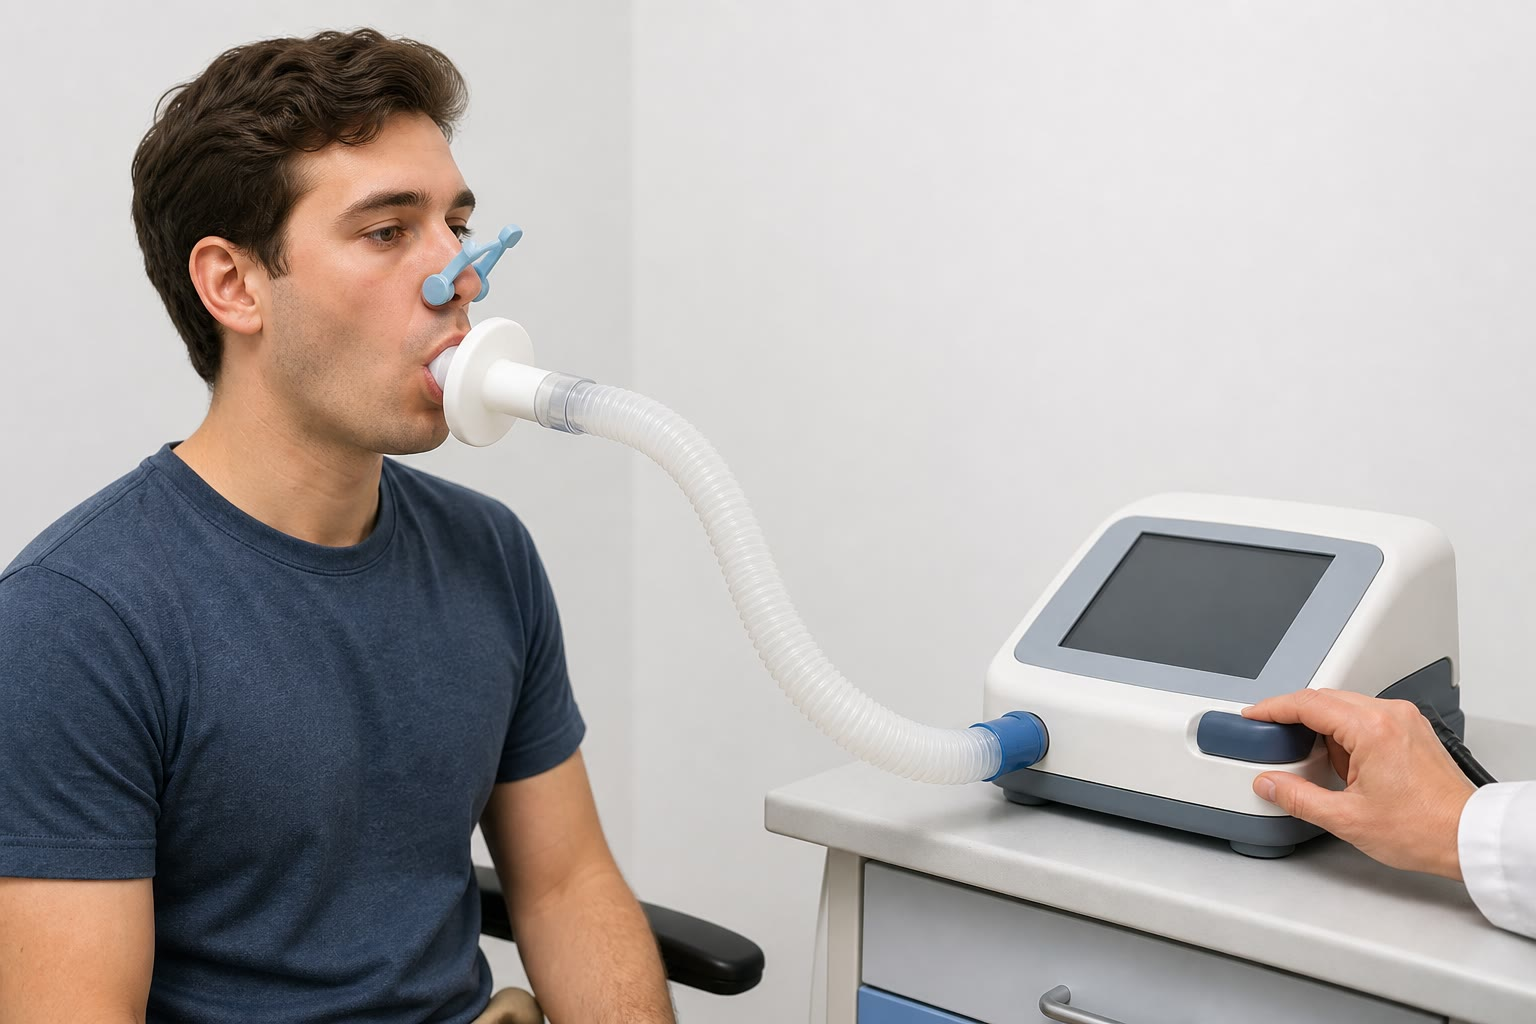
\includegraphics[width=0.58\linewidth]{images/book2/ai/g10-lungs-spirometer.jpg}

{\small قياس الحجوم الرئوية: يتنفس الشخص عبر قطعة فموية في مقياس
تنفسي، وأنفه مشدود بمشبك، والجهاز يسجل حجم كل نفس.}
\end{omfigure}

\section{القلب والدورتان الدمويتان}

\begin{definition}[الصبيب القلبي]\label{def:g10:heart-lungs-effort:output}
القلب مضخة مزدوجة من أربع حجرات. الجانب الأيمن يتلقى الدم العائد من
الأعضاء ويرسله إلى الرئتين (\emph{الدورة الرئوية})؛ والجانب الأيسر
يتلقاه من الرئتين ويرسله إلى الأعضاء (\emph{الدورة العامة}). وصمامات
بين الحجرات وعند المخارج تجعل الجريان في اتجاه واحد. و\emph{الصبيب
القلبي}\index{صبيب قلبي} $Q$ هو حجم الدم الذي يضخه كل جانب في
الدقيقة: أي الحجم المقذوف في النبضة، وهو \emph{الحجم النفضي} $V_s$،
مضروبًا في \emph{التواتر القلبي} $f$،
\[
Q = f \times V_s .
\]
وفي الراحة، $70$ نبضة في الدقيقة من \qty{70}{mL}: أي نحو
\qty{5}{L/min} --- أي حجم الدم كله مرة في الدقيقة.
\end{definition}

\begin{omfigure}
\begin{tikzpicture}[>=Stealth, font=\small,
  ch/.style={draw, thick, rounded corners, minimum width=1.9cm, minimum height=1.0cm, align=center},
  org/.style={draw, thick, rounded corners, minimum width=2.6cm, minimum height=1.0cm, align=center}]
  \node[org, fill=omDef!15] (lungs) at (3.5,3.6) {الرئتان};
  \node[ch, fill=omDef!25] (ra) at (0.7,1.2) {الأذين\\ الأيمن};
  \node[ch, fill=omDef!25] (rv) at (0.7,0) {البطين\\ الأيمن};
  \node[ch, fill=omThm!20] (la) at (6.3,1.2) {الأذين\\ الأيسر};
  \node[ch, fill=omThm!20] (lv) at (6.3,0) {البطين\\ الأيسر};
  \node[org, fill=omThm!12] (org) at (3.5,-2.8) {العضلات\\ وسائر الأعضاء};
  \draw[->, thick, omDef] (ra) -- (rv);
  \draw[->, thick, omDef, rounded corners=6pt] (rv.west) -- (-1.55,0) -- (-1.55,3.6) -- (lungs.west);
  \node[anchor=east, align=right, omDef] at (-1.7,2.4) {الشريان\\ الرئوي};
  \draw[->, thick, omThm, rounded corners=6pt] (lungs.east) -- (8.6,3.6) -- (8.6,1.2) -- (la.east);
  \node[anchor=west, align=left, omThm] at (8.75,2.4) {الأوردة\\ الرئوية};
  \draw[->, thick, omThm] (la) -- (lv);
  \draw[->, thick, omThm, rounded corners=6pt] (lv.east) -- (8.6,0) -- (8.6,-2.8) -- (org.east);
  \node[anchor=west, omThm] at (8.75,-1.4) {الأبهر};
  \draw[->, thick, omDef, rounded corners=6pt] (org.west) -- (-2.3,-2.8) -- (-2.3,1.2) -- (ra.west);
  \node[anchor=east, omDef] at (-2.45,-1.4) {الأوردة};
  \node[font=\small, anchor=north, text width=3.2cm, align=center] at (3.5,-3.6) {أكسجين يخرج، $\mathrm{CO_2}$ يدخل};
  \node[font=\small, anchor=south, text width=3.2cm, align=center] at (3.5,4.2) {أكسجين يدخل، $\mathrm{CO_2}$ يخرج};
  \draw[thick, dashed, gray] (3.5,2.5) -- (3.5,-1.9);
\end{tikzpicture}

{\small الدورة المزدوجة. بالأزرق: دم فقير بالأكسجين، يضخه القلب الأيمن
إلى الرئتين. وبالأحمر: دم غني بالأكسجين، يضخه القلب الأيسر إلى
الأعضاء. والجانبان ينبضان معًا ويضخان الحجم نفسه في الدقيقة.}
\end{omfigure}

\begin{proposition}[الصبيب القلبي أثناء الجهد]\label{prop:g10:heart-lungs-effort:output-exercise}
أثناء الجهد يرتفع التواتر القلبي مع الاستطاعة المقدمة، حتى حد أقصى
يقارب $220$ ناقص العمر بالسنين، ويرتفع الحجم النفضي أيضًا، بنحو النصف
عند غير المدرَّب وأكثر عند المدرَّب. وينتقل \omterm{def:g10:heart-lungs-effort:output}{الصبيب القلبي} عند شاب
بالغ من \qty{5}{L/min} في الراحة إلى \qtyrange{20}{25}{L/min} عند
الجهد الأقصى، وإلى \qty{35}{L/min} أو أكثر عند بطل في رياضات التحمل
يتجاوز حجمه النفضي \qty{180}{mL}.
\end{proposition}
\admitted

\begin{omfigure}
\begin{tikzpicture}
\begin{axis}[
  width=0.86\linewidth, height=5.8cm,
  axis x line=bottom, axis y line=left,
  xmin=0, xmax=320, ymin=0, ymax=210,
  xlabel={الاستطاعة الميكانيكية (W)}, ylabel={التواتر القلبي (في الدقيقة)، الحجم النفضي (mL)},
  xlabel style={font=\small, at={(axis description cs:0.5,-0.12)}, anchor=north},
  ylabel style={font=\small},
  tick label style={font=\small},
  xtick={0,50,100,150,200,250,300}, ytick={0,50,100,150,200},
  legend style={at={(0.5,-0.3)}, anchor=north, legend columns=3, font=\small, draw=none},
  clip=false,
]
\addplot[thick, omThm, mark=*, mark size=1.5pt] coordinates
  {(0,70) (50,95) (100,120) (150,145) (200,170) (250,190) (300,198)};
\addplot[thick, omDef, mark=square*, mark size=1.5pt] coordinates
  {(0,70) (50,90) (100,105) (150,112) (200,115) (250,115) (300,115)};
\addplot[thick, omMeth, dashed, mark=triangle*, mark size=1.8pt] coordinates
  {(0,4.9) (50,8.6) (100,12.6) (150,16.2) (200,19.6) (250,21.9) (300,22.8)};
\legend{{التواتر القلبي}, {الحجم النفضي}, {الصبيب (L/min)}}
\end{axis}
\end{tikzpicture}

{\small التواتر القلبي والحجم النفضي \omterm{def:g10:heart-lungs-effort:output}{والصبيب القلبي} عند شاب في العشرين
باستطاعة متزايدة. الحجم النفضي يستوي عند جهد معتدل؛ وفوق ذلك يرتفع
الصبيب بالتواتر وحده، والتواتر نفسه يستوي قرب $220 - 20 = 200$.}
\end{omfigure}

\begin{example}[الصبيب عند \qty{200}{W}]\label{ex:g10:heart-lungs-effort:output200}
من الشكل: $f = 170$ في الدقيقة، و$V_s = \qty{115}{mL}$، ومنه
$Q = 170 \times 0.115 \approx \qty{19.6}{L/min}$: أي أربعة أمثال صبيب
الراحة. فالقلب يحرك حجم دم الجسم كله أربع مرات في الدقيقة.
\end{example}

\section{إيصال الدم إلى حيث يحتاج إليه}

\begin{proposition}[إعادة توزيع الجريان الدموي]\label{prop:g10:heart-lungs-effort:redistribution}
في الراحة تتلقى العضلات نحو خمس \omterm{def:g10:heart-lungs-effort:output}{الصبيب القلبي}؛ ويأخذ المعي والكبد
والكليتان النصف. وأثناء الجهد الشديد تتسع الشرايين الصغيرة في العضلات
العاملة وتضيق شرايين المعي والكليتين: فتتلقى العضلات عندئذ أكثر من
أربعة أخماس صبيب تضاعف هو نفسه أربع مرات --- أي نحو \qty{20}{L/min}
بدل \qty{1}{L/min}، أي عشرين ضعفًا. ويبقى نصيب الدماغ ثابتًا بالقيمة
المطلقة، ويرتفع نصيب الجلد لحمل الحرارة بعيدًا.
\end{proposition}
\admitted

\begin{omfigure}
\begin{tikzpicture}
\begin{axis}[
  xbar stacked, bar width=15pt,
  width=0.86\linewidth, height=3.8cm,
  axis x line=bottom, axis y line=left,
  xmin=0, xmax=25, xlabel={الجريان الدموي (L/min)},
  xlabel style={font=\small, at={(axis description cs:0.5,-0.3)}, anchor=north},
  symbolic y coords={راحة, جهد أقصى},
  ytick=data, tick label style={font=\small},
  enlarge y limits=0.5,
  legend style={at={(0.5,-0.65)}, anchor=north, legend columns=5, font=\small, draw=none},
]
\addplot[fill=omThm!50, draw=omThm] coordinates {(1.0,راحة) (20.5,جهد أقصى)};
\addplot[fill=omProp!50, draw=omProp] coordinates {(2.5,راحة) (0.9,جهد أقصى)};
\addplot[fill=omDef!50, draw=omDef] coordinates {(0.75,راحة) (0.75,جهد أقصى)};
\addplot[fill=gray!40, draw=gray] coordinates {(0.5,راحة) (1.2,جهد أقصى)};
\addplot[fill=omMeth!50, draw=omMeth] coordinates {(0.25,راحة) (0.65,جهد أقصى)};
\legend{{العضلات}, {المعي والكليتان}, {الدماغ}, {الجلد}, {غير ذلك}}
\end{axis}
\end{tikzpicture}

{\small أين يذهب \omterm{def:g10:heart-lungs-effort:output}{الصبيب القلبي}، في الراحة (\qty{5}{L/min}) وعند الجهد
الأقصى (\qty{24}{L/min}). نصيب العضلات ينتقل من الخمس إلى أكثر من
أربعة أخماس؛ ويحتفظ الدماغ بجريان \qty{0.75}{L/min} طوال الوقت.}
\end{omfigure}

\begin{proposition}[إيصال الأكسجين واستخلاصه]\label{prop:g10:heart-lungs-effort:extraction}
كل لتر من الدم الشرياني يحمل نحو \qty{200}{mL} من الأكسجين، وكله
تقريبًا مرتبط بهيموغلوبين الكريات الحمراء. وفي الراحة تنزع الأعضاء
نحو \qty{50}{mL} من كل لتر؛ وأثناء الجهد تنزع العضلات العاملة حتى
\qty{150}{mL}، أي ثلاثة أمثال. والأكسجين المستهلك في الدقيقة هو
\omterm{def:g10:heart-lungs-effort:output}{الصبيب القلبي} مضروبًا في المقدار المنزوع من كل لتر --- فارتفاع الصبيب
خمسة أمثال وارتفاع الاستخلاص ثلاثة أمثال يعطيان معًا ارتفاع استهلاك
الأكسجين خمسة عشر ضعفًا في \cref{ch:g10:exercise-and-energy}.
\end{proposition}
\admitted

\begin{example}[التحقق من ميزانية الأكسجين]\label{ex:g10:heart-lungs-effort:fick}
الراحة: \qty{5}{L/min} $\times$ \qty{50}{mL/L} $= \qty{250}{mL/min}$،
وهو استهلاك الراحة. والجهد الأقصى عند تلميذ مدرَّب:
\qty{23}{L/min} $\times$ \qty{150}{mL/L} $= \qty{3.45}{L/min}$ ---
أي $\dot V\!\mathrm{O_2}$max يبلغ \qty{50}{mL/min} لكل كيلوغرام عند
\qty{69}{kg}، وهو رقم الفصل السابق بالضبط.
\end{example}

\section{كيف تضبط الاستجابة}

\begin{proposition}[الضبط العصبي والهرموني]\label{prop:g10:heart-lungs-effort:control}
تقود القلبَ وعضلاتِ التنفس مراكزُ عصبية في قاعدة الدماغ. وتبلغ القلبَ
مجموعتان من الأعصاب: واحدة تبطئه وهي نشطة في الراحة؛ وأخرى تسرّعه
وتقوي كل نبضة. وعند بدء الجهد ينسخ أمر الدماغ إلى العضلات إلى تلك
المراكز --- فيتسارع القلب في غضون نبضة أو نبضتين --- وتبلّغ مستقبلات
في العضلات والمفاصل عن الحركة. ثم، مع استمرار الجهد، تقيس مستقبلات في
الشرايين ثاني أكسيد الكربون وحموضة الدم وتضبط \omterm{def:g10:heart-lungs-effort:ventilation}{التهوية} والتواتر القلبي
لتبقيهما قرب قيمتي الراحة. وتضيف الغدتان الكظريتان هرمون
\emph{الأدرينالين}\index{أدرينالين}، وهو يعزز التسارع ويوسّع شرايين
العضلات.
\end{proposition}
\begin{proof}[شواهد]
قطع العصب المبطئ عند حيوان يرفع تواتره القلبي في الراحة من 70 إلى نحو
100؛ وتنبيهه يوقف القلب. وتنبيه العصب المسرّع يضاعف التواتر. والشخص
الذي يقال له إن جهدًا ينتظره يبين تواترًا قلبيًا مرتفعًا قبل أن يتحرك؛
والشخص الذي يتنفس هواءً غنيًا بثاني أكسيد الكربون يزيد تهويته في غضون
دقيقة، والشخص الذي يبقى ثاني أكسيد الكربون في دمه ثابتًا اصطناعيًا
أثناء الجهد يزيدها أيضًا عند بدء الحركة --- فالآليتان، الاستباق
والتصحيح، حقيقيتان كلتاهما.
\end{proof}

\begin{method}[حساب إيصال الأكسجين]\label{met:g10:heart-lungs-effort:compute}
\begin{enumerate}
  \item \omterm{def:g10:heart-lungs-effort:ventilation}{التهوية}: الحجم الجاري $\times$ التواتر. ولا يبلغ الأسناخَ إلا
        نحو 70\% من كل نفس؛ أما الباقي فيملأ الطرق الهوائية.
  \item \omterm{def:g10:heart-lungs-effort:output}{الصبيب القلبي}: $Q = f \times V_s$، باللترات في الدقيقة إذا
        كان $V_s$ باللترات.
  \item الأكسجين المستهلك في الدقيقة: $Q \times$ (الأكسجين المنزوع من
        لتر الدم).
  \item الجريان إلى عضو: نصيبه من $Q$. وقارن الجريانات المطلقة، لا
        الأنصبة --- فنصيب أصغر من صبيب أكبر قد يكون دمًا أكثر.
  \item تحقق: الاستهلاك لا يستطيع تجاوز $\dot V\!\mathrm{O_2}$max،
        و$f$ لا يستطيع تجاوز نحو $220 - $ العمر.
\end{enumerate}
\end{method}

\begin{remark}[أين يقع الحد]\label{rem:g10:heart-lungs-effort:limit}
\omterm{def:g10:heart-lungs-effort:ventilation}{التهوية} تستطيع تجاوز \qty{150}{L/min} والدم المغادر للرئتين يكاد يكون
مشبعًا عند الجهد الأقصى: فالرئتان ليستا عنق الزجاجة. وإنما هو الحجم
النفضي: فهو يحدد كم دم، ومن ثم كم أكسجين، توصله كل نبضة. وتدريب التحمل
يكبّر القلب وحجمه النفضي --- ولذلك ينبض قلب مدرَّب في الراحة عند 45
بدل 70 لأجل \qty{5}{L/min} نفسها، ولذلك يرتفع
$\dot V\!\mathrm{O_2}$max بالتدريب.
\end{remark}

\section{تمارين}

\begin{exercise}[$\star$]\label{exo:g10:heart-lungs-effort:1}
احسب \omterm{def:g10:heart-lungs-effort:ventilation}{تهوية} شخص يتنفس \qty{0.6}{L} أربع عشرة مرة في الدقيقة؛ ثم \omterm{def:g10:heart-lungs-effort:ventilation}{تهوية}
الشخص نفسه وهو يتنفس \qty{2.2}{L} خمسًا وثلاثين مرة في الدقيقة.
\end{exercise}

\begin{exercise}[$\star$]\label{exo:g10:heart-lungs-effort:2}
عرّف \omterm{def:g10:heart-lungs-effort:output}{الصبيب القلبي} وأعطِ صيغته. واحسبه لتواتر قلبي قدره 65 في الدقيقة
وحجم نفضي قدره \qty{75}{mL}.
\end{exercise}

\begin{exercise}[$\star$]\label{exo:g10:heart-lungs-effort:3}
تتبّع مسار كرية حمراء من الأذين الأيمن رجوعًا إلى الأذين الأيمن، مسميًا
الحجرات والدورتين.
\end{exercise}

\begin{exercise}[$\star$]\label{exo:g10:heart-lungs-effort:4}
من شكل المخطط التنفسي، أعطِ الحجم الجاري والسعة الحيوية والحجم
المتبقي.
\end{exercise}

\begin{exercise}[$\star$]\label{exo:g10:heart-lungs-effort:5}
ما التواتر القلبي الأقصى عند ابن 16 سنة؟ وعند ابن 60 سنة؟
\end{exercise}

\begin{exercise}[$\star\star$]\label{exo:g10:heart-lungs-effort:6}
من شكل التواتر القلبي، احسب \omterm{def:g10:heart-lungs-effort:output}{الصبيب القلبي} عند \qty{100}{W} وعند
\qty{300}{W}، والعامل بينهما.
\end{exercise}

\begin{exercise}[$\star\star$]\label{exo:g10:heart-lungs-effort:7}
في الراحة يتلقى المعي والكليتان 50\% من \qty{5}{L/min}؛ وعند الجهد
الأقصى 4\% من \qty{24}{L/min}. احسب الجريانين. وأيهما يتغير أكثر،
النصيب أم الجريان المطلق؟
\end{exercise}

\begin{exercise}[$\star\star$]\label{exo:g10:heart-lungs-effort:8}
شخص صبيبه القلبي \qty{18}{L/min} وعضلاته تنزع \qty{140}{mL} من
الأكسجين لكل لتر. احسب استهلاكه من الأكسجين. وهل هو قريب من سقف تلميذ
مدرَّب؟
\end{exercise}

\begin{exercise}[$\star\star$]\label{exo:g10:heart-lungs-effort:9}
لماذا يبقى جريان الدم إلى الدماغ عند \qty{0.75}{L/min} بينما يقطع
ثلثا جريان المعي أثناء الجهد؟ فكّر فيما يحتمله كل عضو.
\end{exercise}

\begin{exercise}[$\star\star$]\label{exo:g10:heart-lungs-effort:10}
دراجة مدرَّبة تواترها القلبي في الراحة 42 وصبيبها في الراحة
\qty{5}{L/min}. احسب حجمها النفضي وقارنه بحجم شخص غير مدرَّب.
\end{exercise}

\begin{exercise}[$\star\star$]\label{exo:g10:heart-lungs-effort:11}
فسّر لماذا يبدأ التواتر القلبي بالارتفاع قبل الخطوة الأولى في سباق،
وماذا كان ليحدث لعدّاء لا يعمل ضبطه إلا بتحسس ثاني أكسيد كربون الدم.
\end{exercise}

\begin{exercise}[$\star\star\star$]\label{exo:g10:heart-lungs-effort:12}
شخصان يبلغان التواتر القلبي الأقصى نفسه، وهو 195. لأحدهما حجم نفضي
أقصى \qty{110}{mL}، وللآخر \qty{160}{mL}. وباستخلاص أكسجين واحد قدره
\qty{150}{mL/L}، احسب استهلاكهما الأقصى للأكسجين، وقل بم يتنبأ
\cref{rem:g10:heart-lungs-effort:limit} عن تاريخهما التدريبي.
\end{exercise}

\begin{exercise}[$\star\star\star$]\label{exo:g10:heart-lungs-effort:13}
الهواء 21\% أكسجين. شخص يهوّي \qty{100}{L/min} عند الجهد الأقصى
ويستهلك \qty{3.5}{L/min} من الأكسجين. فأي نسبة من الأكسجين الذي
يستنشقه يستعمله فعلًا؟ وماذا يفعل الباقي؟
\end{exercise}

\begin{exercise}[$\star\star\star$]\label{exo:g10:heart-lungs-effort:14}
دواء يحصر الأعصاب المسرّعة وأثر \omterm{prop:g10:heart-lungs-effort:control}{الأدرينالين} في القلب، فيحد التواتر
القلبي عند 110. تنبأ بأثره في \omterm{def:g10:heart-lungs-effort:output}{الصبيب القلبي} عند الجهد الأقصى، وفي
$\dot V\!\mathrm{O_2}$max، وفيما يستطيع المريض فعله.
\end{exercise}

\begin{exercise}[$\star\star\star$]\label{exo:g10:heart-lungs-effort:15}
شخص على ارتفاع عال دمه الشرياني يحمل \qty{150}{mL} من الأكسجين لكل لتر
بدل \num{200}. فمع \omterm{def:g10:heart-lungs-effort:output}{الصبيب القلبي} الأقصى نفسه والاستخلاص نفسه البالغ
75\% من الأكسجين الموصل، احسب الخسارة في $\dot V\!\mathrm{O_2}$max
بالمئة. واقترح تكيفًا واحدًا يجريه الجسم في الأسابيع التالية.
\end{exercise}

\section{مسألة: اختبار الجهد}

\begin{problem}[{مسألة نهاية الأسبوع --- اختبار جهد عند طبيب قلب:
تواتر قلبي وحجم نفضي وتهوية واستخلاص أكسجين تقاس عند استطاعة متزايدة،
والمضاعفة التي تحققها مجتمعة}]
\label{pb:g10:heart-lungs-effort:1}
توم، 17 سنة، كتلته \qty{68}{kg}، يدوس على دراجة مختبرية بينما يسجل
تواتره القلبي وتهويته وهواؤه الزفيري. والنتائج:

\begin{center}
\begin{tabular}{lccccc}
الاستطاعة (W) & 0 & 75 & 150 & 225 & 300 \\ \hline
التواتر القلبي (في الدقيقة) & 62 & 105 & 140 & 175 & 198 \\
الحجم النفضي (mL) & 72 & 100 & 116 & 120 & 120 \\
الحجم الجاري (L) & 0.5 & 1.2 & 1.8 & 2.3 & 2.6 \\
الأنفاس في الدقيقة & 13 & 18 & 24 & 32 & 44 \\
$\mathrm{O_2}$ المنزوع من لتر الدم (mL) & 52 & 90 & 120 & 145 & 155 \\
\end{tabular}
\end{center}

\medskip
\noindent\textbf{الجزء الأول --- القلب.}
\begin{enumerate}
  \item احسب صبيب توم القلبي عند كل استطاعة.
  \item بأي عامل ارتفع الصبيب عند \qty{300}{W}؟ وأي جزء من ذلك العامل
        يأتي من التواتر وأي جزء من الحجم النفضي؟
  \item فوق أي استطاعة يكف الحجم النفضي عن الارتفاع؟ وما الذي يزيد
        الصبيب وحده وراء ذلك؟
  \item قارن التواتر القلبي الأقصى عند توم بالقاعدة التقريبية.
  \item صبيبه في الراحة نحو \qty{4.5}{L/min}. فإذا كان حجم دمه
        \qty{5}{L}، فكم تستغرق دورة كاملة واحدة في الراحة، وعند
        \qty{300}{W}؟
\end{enumerate}

\medskip
\noindent\textbf{الجزء الثاني --- الرئتان.}
\begin{enumerate}[resume]
  \item احسب \omterm{def:g10:heart-lungs-effort:ventilation}{التهوية} عند كل استطاعة.
  \item بأي عامل ارتفعت عند \qty{300}{W}؟ وأي العاملين، الحجم أم
        التواتر، يسهم أكثر؟
  \item السعة الحيوية عند توم \qty{5.0}{L}. فأي نسبة منها يستعملها كل
        نفس عند \qty{300}{W}؟
  \item ارتفعت \omterm{def:g10:heart-lungs-effort:ventilation}{التهوية} بعامل أكبر من عامل \omterm{def:g10:heart-lungs-effort:output}{الصبيب القلبي}. فهل يعني ذلك
        أن الرئتين تحدان الأداء؟ استعمل
        \cref{rem:g10:heart-lungs-effort:limit}.
  \item لا يبلغ الأسناخَ إلا 70\% من كل نفس. احسب \omterm{def:g10:heart-lungs-effort:ventilation}{التهوية} السنخية في
        الراحة وعند \qty{300}{W}.
\end{enumerate}

\medskip
\noindent\textbf{الجزء الثالث --- الأكسجين.}
\begin{enumerate}[resume]
  \item احسب استهلاك توم من الأكسجين عند كل استطاعة، من \omterm{def:g10:heart-lungs-effort:output}{الصبيب القلبي}
        والأكسجين المنزوع من كل لتر.
  \item عبّر عن القيمة عند \qty{300}{W} بالمليلترات في الدقيقة لكل
        كيلوغرام. أهي $\dot V\!\mathrm{O_2}$max، ولأي صنف من الأشخاص؟
  \item بأي عامل ارتفع الاستهلاك من الراحة إلى \qty{300}{W}؟ فصّله
        إلى عامل من القلب وعامل من الاستخلاص.
  \item باستعمال \qty{20}{kJ} لكل لتر أكسجين، احسب الاستطاعة
        الاستقلابية عند \qty{300}{W} ومردود العضلات (الاستطاعة
        الميكانيكية مقسومة على الاستطاعة الاستقلابية فوق الراحة).
  \item ارسم، أو صف، استهلاك الأكسجين بدلالة الاستطاعة الميكانيكية.
        أهو خطي؟ وأين السقف؟
\end{enumerate}

\medskip
\noindent\textbf{الجزء الرابع --- الضبط والحكم.}
\begin{enumerate}[resume]
  \item بلغ تواتر توم القلبي 75 وهو جالس ينتظر بدء الاختبار. فسّر.
  \item عند \qty{300}{W} يبقى دمه الشرياني مشبعًا بالأكسجين بنسبة
        95\%. فما الذي يعلمك إياه ذلك عن تبادل الأسناخ، وعن موضع الحد
        في $\dot V\!\mathrm{O_2}$max عنده؟
  \item يلاحظ طبيب القلب أن العضلات تتلقى الآن نحو \qty{20}{L/min} من
        الدم. فأي نسبة من الصبيب هي تلك، وأين ذهب باقي توزيع الراحة؟
  \item بعد ستة أشهر من التدريب صار حجم توم النفضي الأقصى
        \qty{140}{mL} عند التواتر الأقصى والاستخلاص نفسيهما. احسب
        $\dot V\!\mathrm{O_2}$max الجديد عنده.
  \item اذكر النتيجة: الأرقام الثلاثة (القلب والاستخلاص \omterm{def:g10:heart-lungs-effort:ventilation}{والتهوية})
        التي ضاعف بها جسم توم إمداده من الأكسجين في الراحة، وأيها
        غيره التدريب.
\end{enumerate}
\end{problem}
